\chapter{}
\label{chp2:concept_model}

\section{Derivation of the Mathematical Model}
\label{sec:math_model}

$$x_{1}= l_{1}\cos(\theta)$$
$$y_{1} = -l_{1}\sin(\theta)$$

$$x_{2} = L_{1}\sin(\theta) + l_{2}\sin(\theta + \phi)$$
$$y_{2} = -L_{1}\cos(\theta) - l_{2}\cos(\theta + \phi)$$

$$\dot{x_{2}} = L_{1}\cos(\theta)\dot{\theta} - l_{2}\cos(\theta+\phi)(\dot{\theta}+\dot{\phi}) $$
$$\dot{y_{2}} = L_{1}\sin(\theta)\dot{\theta}+l_{2}\sin(\theta+\phi)(\dot{\theta}+\dot{\phi})$$

$$x_{2}^2 = L_{1}^2\cos(\theta)^2\theta^2 +l_{2}^2\cos(\theta+\phi)^2(\dot{\theta}+\dot{\phi})^2 + 2L_{1}l_{2}\dot{\theta}(\dot{\theta}+\dot{\theta})\cos(\theta)\cos(\theta+\phi)$$
$$y_{2}^2 = L_{1}^2\sin(\theta)^2\theta^2 +l_{2}^2\sin(\theta+\phi)^2(\dot{\theta}+\dot{\phi})^2 + 2L_{1}l_{2}\dot{\theta}(\dot{\theta}+\dot{\theta})\sin(\theta)\sin(\theta+\phi)$$

$$x_{2}^2+y_{2}^2 = L_{1}^2\theta^2[\cos(\theta)^2+\sin(\theta)^2]+l_{2}^2(\dot{\theta}+\dot{\phi})^2[\cos(\theta+\phi)^2+\sin(\theta+\phi)^2] +$$
$$ 2L_{1}l_{2}\dot{\theta}(\dot{\theta}+\dot{\phi})[\cos(\theta)\cos(\theta+\phi)+\sin(\theta)\sin(\theta+\phi)]$$	

Using the following trigonometric identities $$ \cos(\gamma)^2 + \sin(\gamma)^2 = 1 $$ 
$$ \cos(\gamma)\cos(\alpha)+\sin(\gamma)\sin(\alpha) = \cos(\gamma - \alpha) $$ the above equation resolves to: $$ V_{2}^2 = L_{1}\dot{\theta}^2+l_{2}^2(\dot{\theta}+\dot{\phi})^2 + 
2L_{1}l_{2}(\dot{\theta}+\dot{\phi})\dot{\theta}\cos(\phi)$$

The kinetic energy in the system consist of the fixed rotation of the underactuated  pendulum and the rotation and velocity of the actuated pendulum.

$$ T = \frac{1}{2}I_{A}\dot{\theta}^2 + \frac{1}{2}I_{B}(\dot{\theta}+\dot{\phi})^2 + \frac{1}{2}m_{2}V_{2}^2$$
$$ T = \frac{1}{2}I_{A}\dot{\theta}^2 + \frac{1}{2}I_{B}(\dot{\theta}+\dot{\phi})^2 + \frac{1}{2}m_{2}[L_{1}\dot{\theta}^2+l_{2}^2(\dot{\theta}+\dot{\phi})^2 + 
2L_{1}l_{2}(\dot{\theta}+\dot{\phi})\dot{\theta}\cos(\phi)]^2$$

The potential energy in the system is defined as
$$V=-m_{1}gl_{1}\cos(\theta)-m_{2}g[L_{1}\cos(\theta)+l_{2}\cos(\theta+\phi)]$$

The Lagrange is defined as 
$$\mathcal{L}=T-V$$
$$\mathcal{L} = \frac{1}{2}I_{A}\dot{\theta}^2 + \frac{1}{2}I_{B}(\dot{\theta}+\dot{\phi})^2 + \frac{1}{2}m_{2}[L_{1}\dot{\theta}^2+l_{2}^2(\dot{\theta}+\dot{\phi})^2 + 
2L_{1}l_{2}(\dot{\theta}+\dot{\phi})\dot{\theta}\cos(\phi)]^2+m_{1}gl_{1}\cos(\theta)+$$
$$m_{2}g[L_{1}\cos(\theta)+l_{2}\cos(\theta+\phi)]$$

$$\frac{\partial\mathcal{L}}{\partial\theta} = -m_{1}gl_{1}\sin(\theta)-m_{2}gL_{2}\sin(\theta)-m_{2}gl_{2}\sin(\theta+\phi)$$
$$\frac{d}{dt}\frac{\partial\mathcal{L}}{\partial\dot{\theta}} = I_{A}\ddot{\theta}+I_{B}\ddot{\theta}+I_{B}\ddot{\phi}+m_{2}L_{1}^2\ddot{\theta}+m_{2}l_{2}^2\ddot{\theta}+m_{2}l_{2}\ddot{\phi}+2m_{2}L_{1}l{2}\ddot{\theta}\cos(\phi)-2m_{2}L_{1}l_{2}\dot{\theta}\dot{\phi}\sin(\phi)+$$
$$m_{2}L_{1}l_{2}\ddot{\phi}\cos(\phi)-m_{2}L_{1}l_{2}\dot{\phi}^2\sin(\phi)$$


$$\frac{\partial\mathcal{L}}{\partial\phi} = -m_{2}L_{1}l_{2}(\dot{\theta}+\dot{\phi})\dot{\theta}\sin(\phi)-m_{2}gl_{2}\sin(\theta+\phi)$$

$$\frac{d}{dt}\frac{\partial\mathcal{L}}{\partial\dot{\phi}}=I_{B}\ddot{\theta}+I_{B}\ddot{\phi}+m_{2}l_{2}^2\ddot{\theta}+m_{2}l_{2}^2\ddot{\phi}+m_{2}L_{1}l_{2}\ddot{\theta}\cos(\phi)-m_{2}L_{1}l_{2}\dot{\theta}\dot{\phi}\sin(\phi)$$

The differential equation describing the dynamics of the system is
$$\frac{d}{dt}\frac{\partial\mathcal{L}}{\partial\vec{\dot{q}}}-\frac{\partial\mathcal{L}}{\partial q} = B(\dot{q})+\tau(q)$$ 
where  $ q = 
\begin{bmatrix}
\theta \\
\phi
\end{bmatrix}
$
\section{Collocated Linearisation}
\begin{equation} \label{app:eq:condense1}
d_{11}\ddot{\theta}+d_{12}\ddot{\phi} + h_{1} + \psi_{1} = 0
\end{equation}
\begin{equation} \label{app:eq:condense2}
d_{21}\ddot{\theta} + d_{22}\ddot{\phi} + h_{2} + \psi_{2} = \tau
\end{equation}

Starting from the condense equation (\ref{app:eq:condense1}) and (\ref{app:eq:condense2}), $\ddot{q_{1}}$ is solved in equation (\ref{app:eq:condense1}) and substituted in (\ref{app:eq:condense1}) resulting in 

\begin{equation} \label{app:eq:condense2}
\bar{d_{2}}\ddot{\theta} + \bar{h_{2}} + \bar{\psi_{2}} = \tau
\end{equation}
where the newly defined terms are given as: 
$$\bar{d_{2}} = d_{22} - \frac{d_{21}d_{12}}{d_{11}}$$
$$\bar{h_{2}} = h_{2} - \frac{d_{21}h_{1}}{d_{11}} $$
$$\bar{\psi_{2}} = \psi_{2} - \frac{d_{21}\psi_{1}}{d_{11}} $$


$\tau$ can now chosen to linearise the terms in equation (\ref{app:eq:condense2}) as:

$\tau = \bar{d_{2}}v_{2}+\bar{h_{2}} + \bar{\psi}$


\section{Taylor Series Expansion Around Unstable Equilibrium Position}
\label{sec:linerisation}






\section{Communication Structure}
\label{sec:software_requirements}
\begin{figure}[h]
	\centering
	\begin{tikzpicture}[cell/.style={rectangle,draw=black},
	space/.style={minimum height=1.5em,matrix of nodes,row sep=-\pgflinewidth,column sep=-\pgflinewidth,column 1/.style={font=\ttfamily}},text depth=0.5ex,text height=2ex,nodes in empty cells]
	

	
	\matrix (first)[space, row 2/.style={minimum width=3em,nodes={cell,minimum width=3.5em}},row 3/.style={nodes={cell,minimum width=2em}}]
	{
		byte &0   & 1  & 2 & 3 & 4& \ldots & n-1&n  \\   
		&\$  & cmd  & , & value & value &  & \textbackslash r &  \textbackslash n \\};
	
	
	
	
\end{tikzpicture}
	\caption{Data Structure for Sending Commands}
	\label{fig:uart_struct_app}
\end{figure}

In Table \ref{table:uart_commands} the various commmands that are used in the command structure shown in Figure \ref{fig:uart_struct_app} used for debugging purposes is explained with the possible value ranges that can be used.


\begin{table}[h]
	\centering
	\begin{tabular}{|c|c|c|c|}
		\hline
		Command & Range &  Reason for Implementation & Effect \\
		\hline
		\hline
		A & None & Testing of the UART circuit & Send the following text: Feedback Control Of Robotic Gymnast\\
		\hline
		B & 0-100 &  & Changes PWM Duty-Cycle \\
		\hline
		C & 0-1 & Testing of AND digital Circuit Directional Control of Motor & Change the rotational direction \\
		\hline
		D & & & \\
		\hline
	
	\end{tabular}
	\caption{Summary of Communication Commands and their Effects}
	\label{table:uart_commands}

\end{table}


\newpage

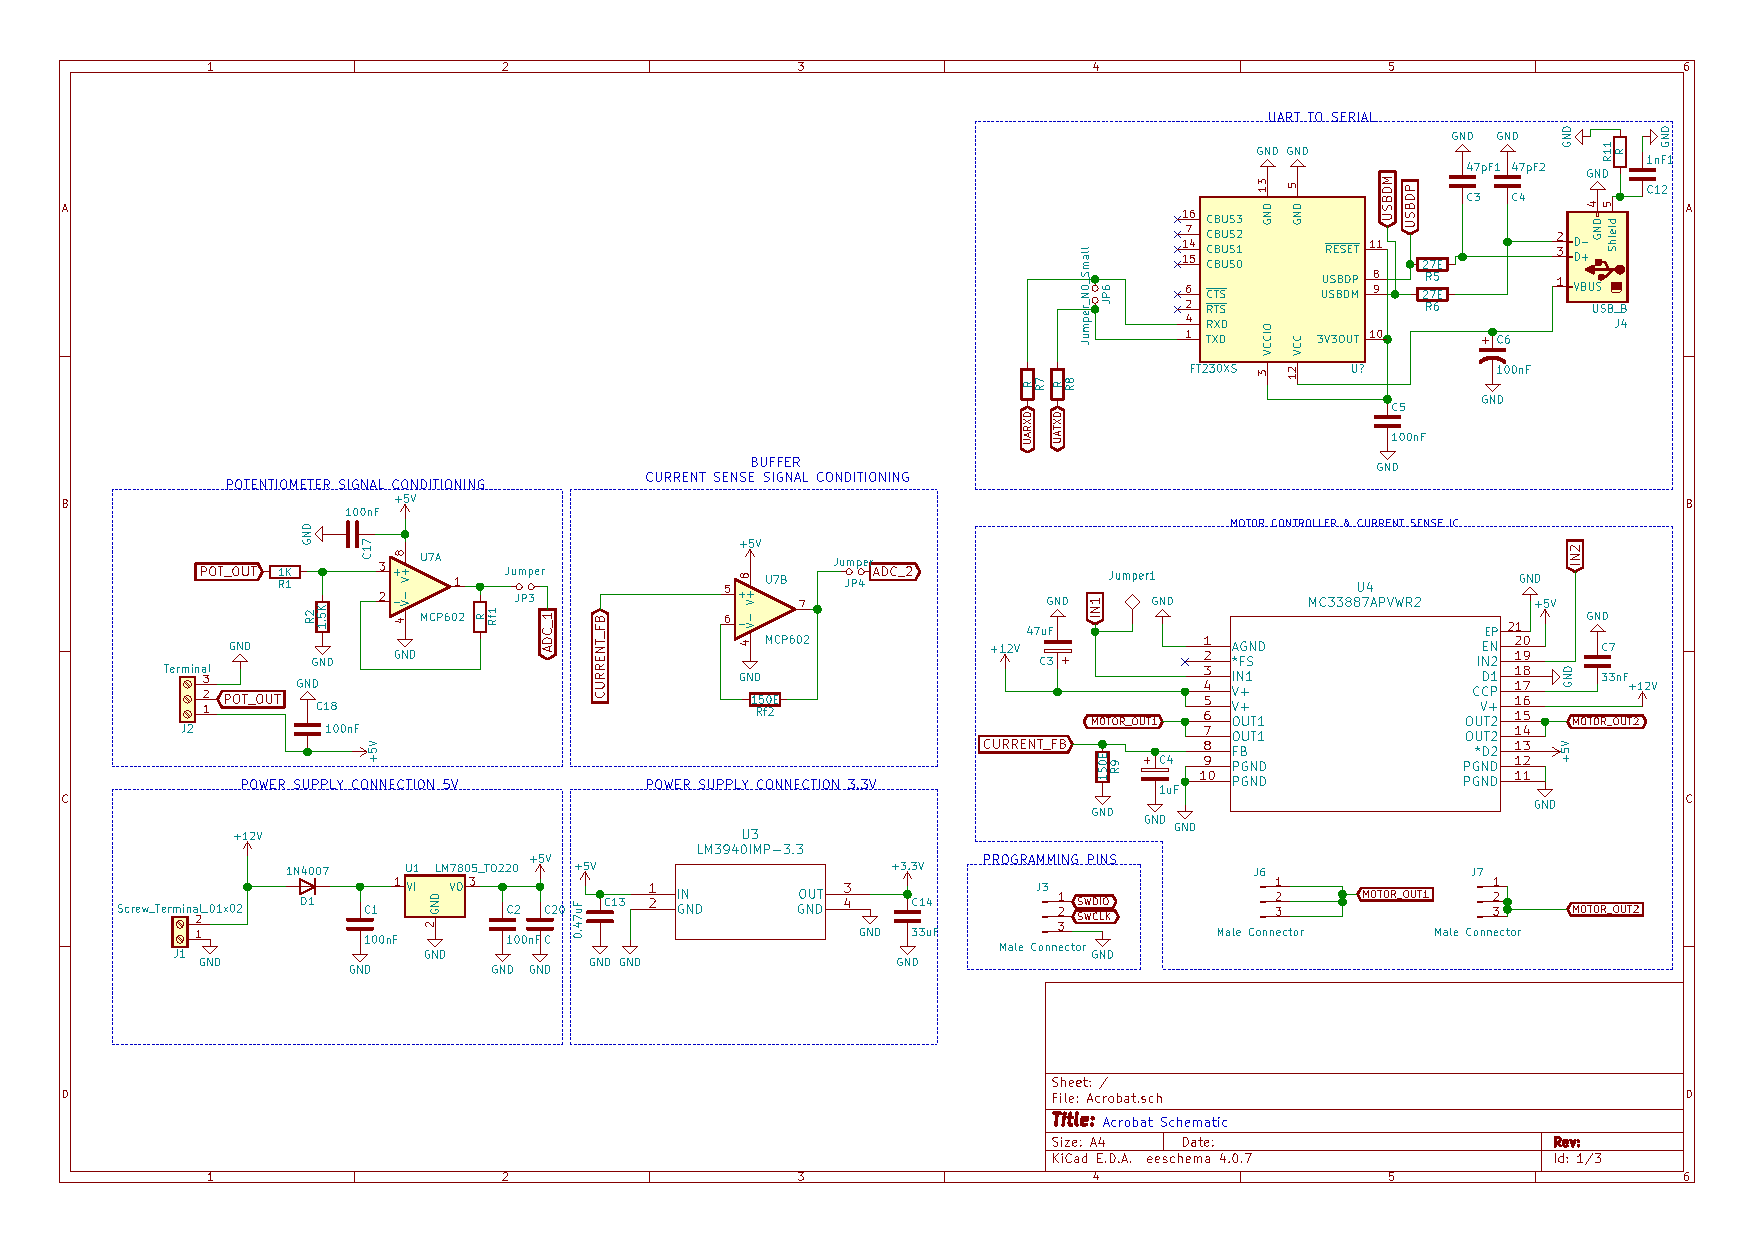
\includepdf[pages=1,pagecommand={\section{Electronic Design Schematic} \thispagestyle{empty} \label{sec:schematics}}, fitpaper=true]{./figs/Acrobat.pdf}
\includepdf[pages=2-,pagecommand={\thispagestyle{empty}}, fitpaper=true]{./figs/Acrobat.pdf}
%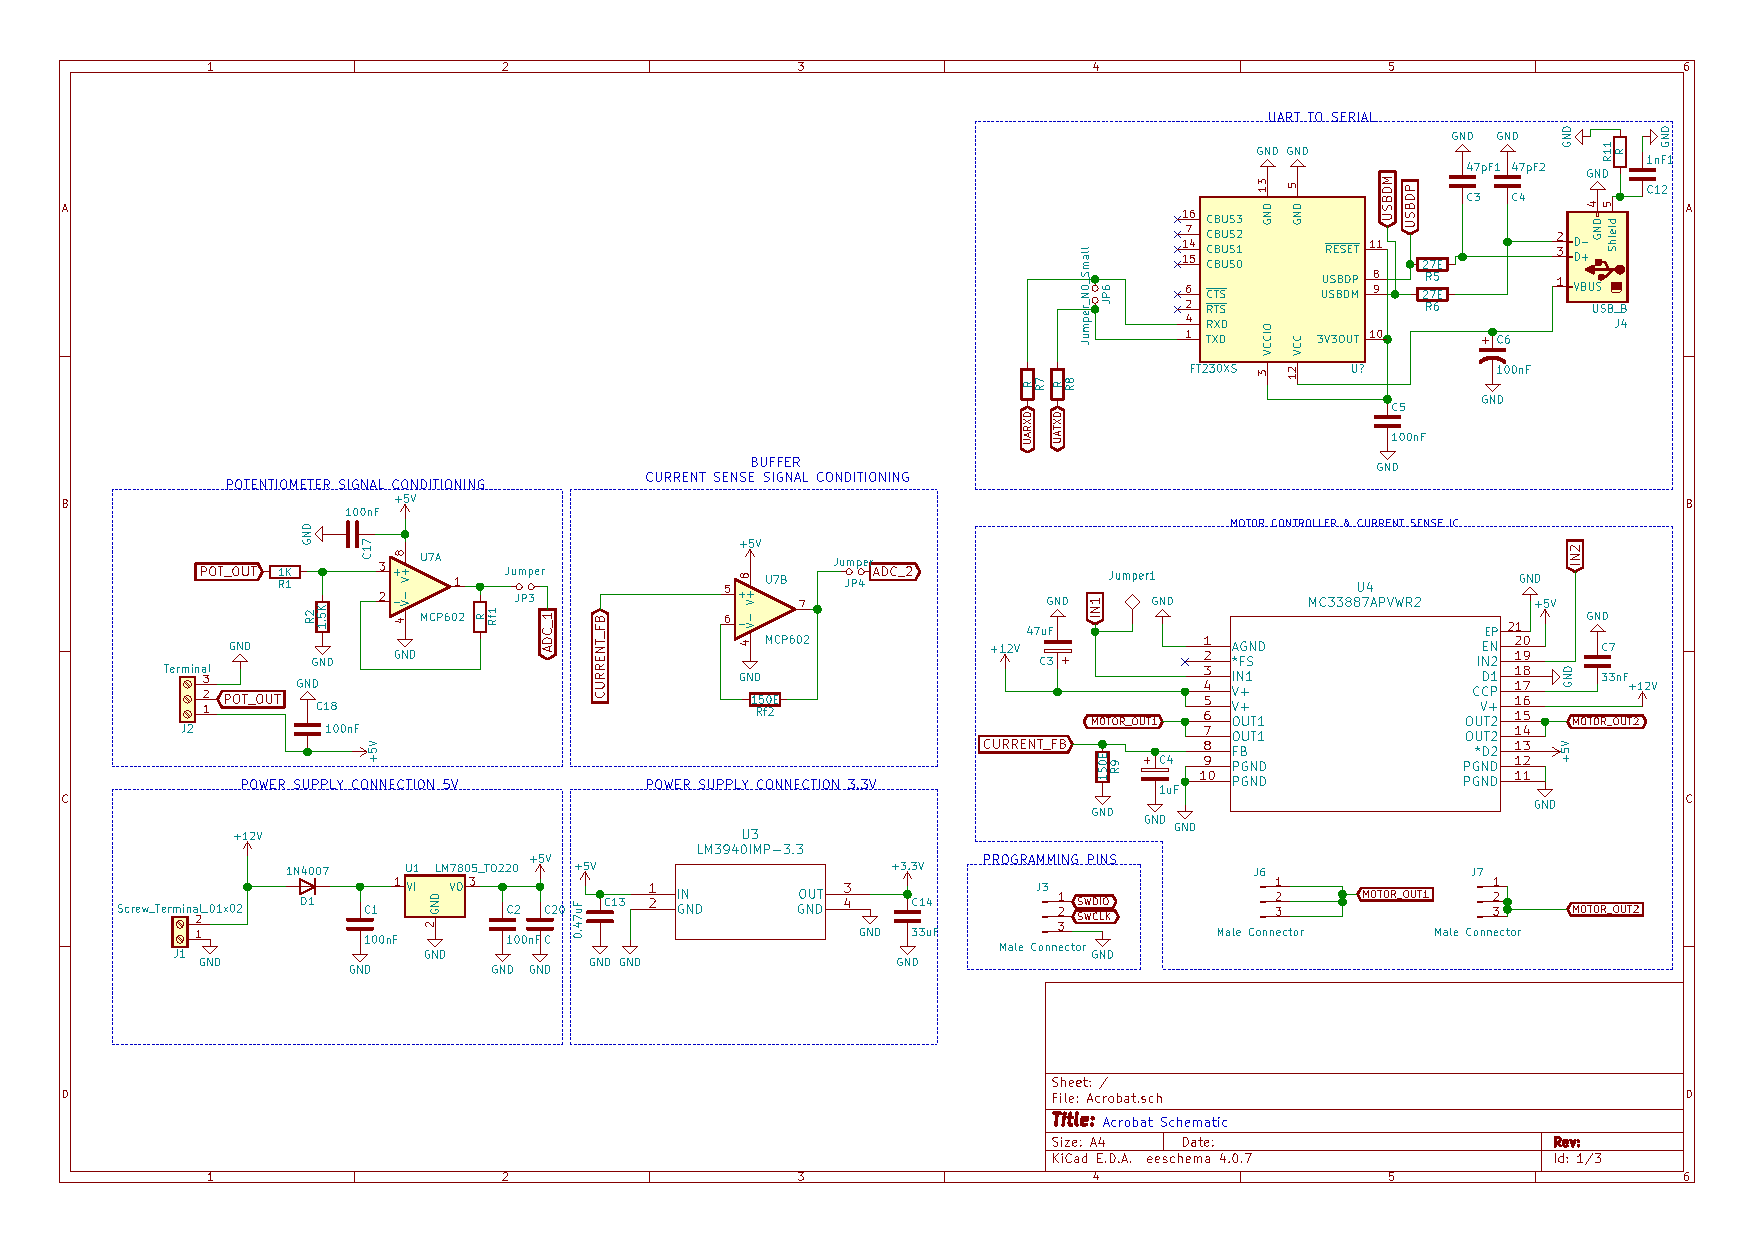
\includepdf[pages=-,scale-=0.8]{./figs/Acrobat.pdf}
%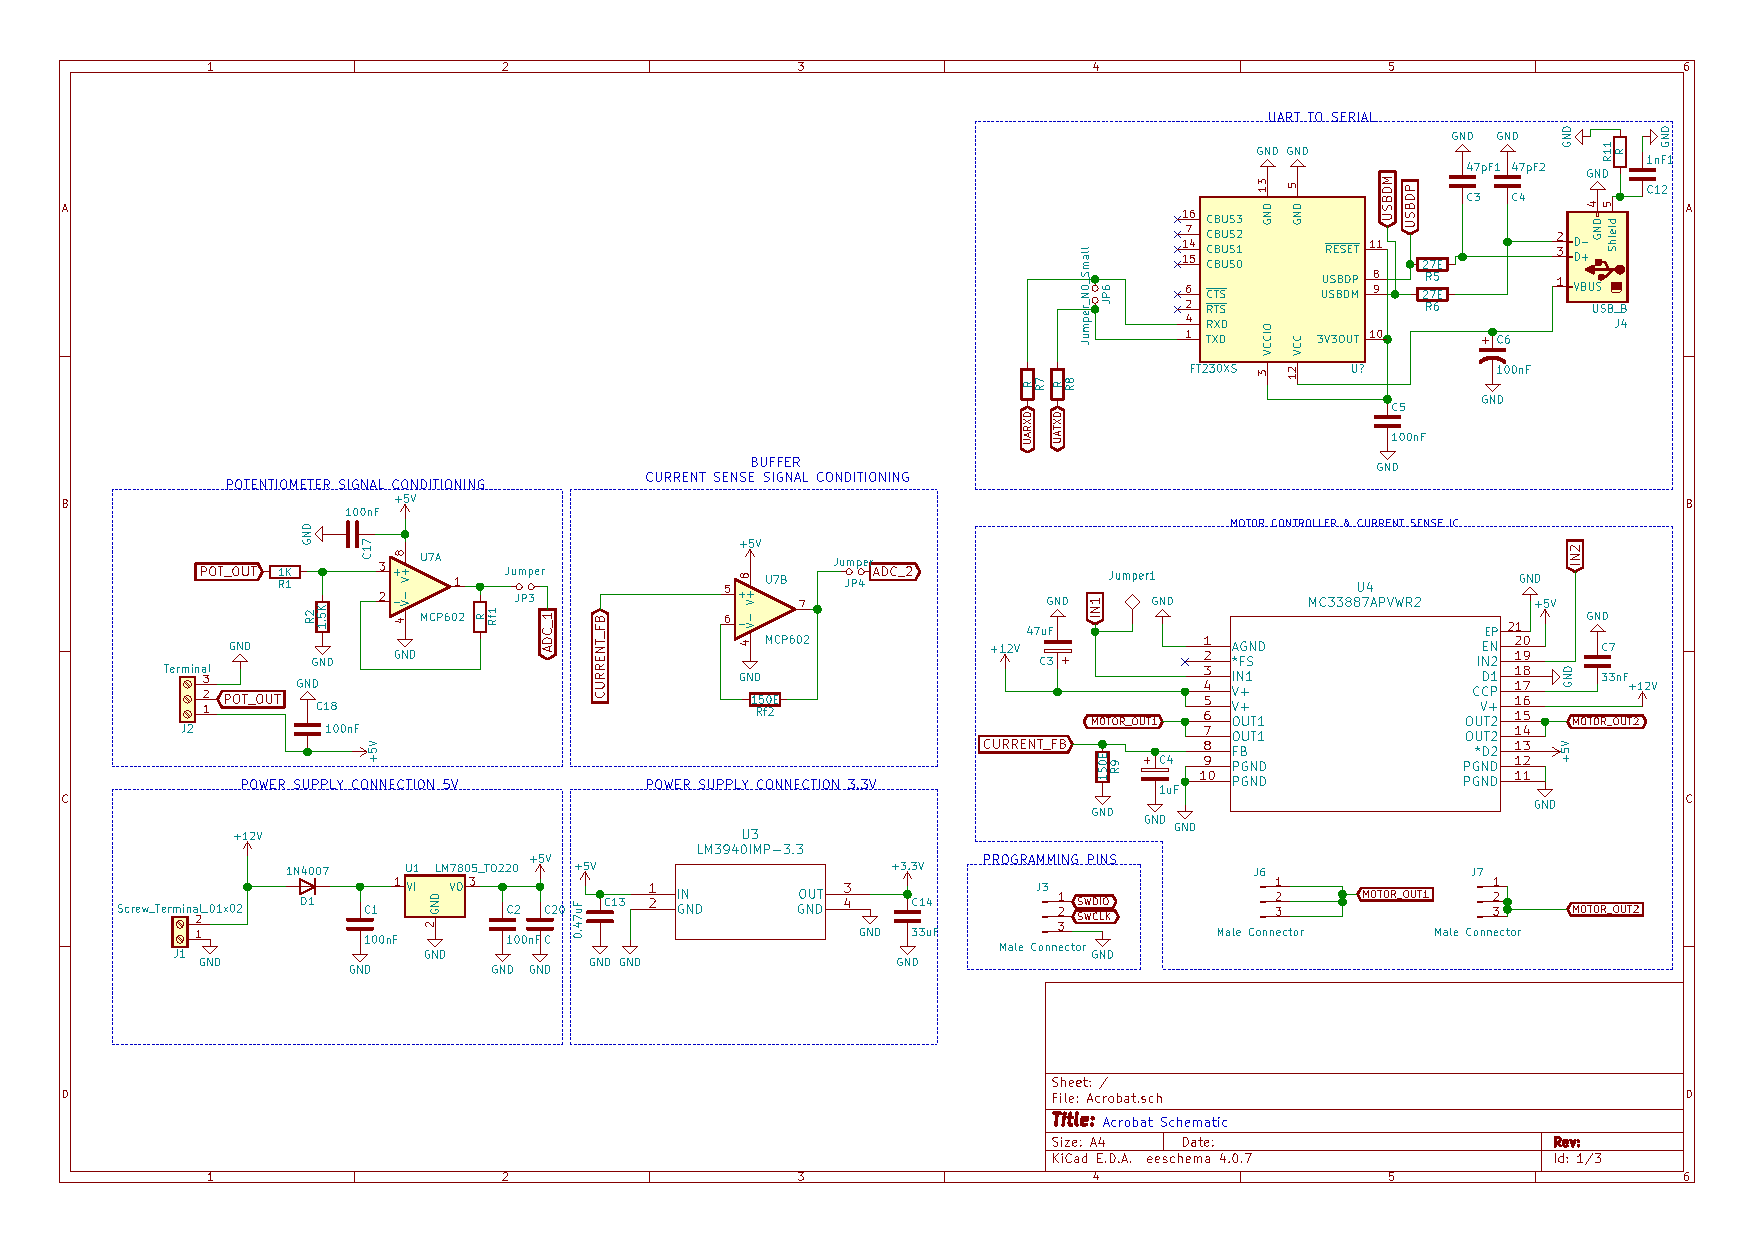
\includegraphics{./figs/Acrobat.pdf}

\section{Techno-Economy Assessment}

\subsection{Budget}
The comparison between the proposed and actual budget is discussed, why additional expenses occurred and where was savings possible.  


\subsection{Planning}
\subsection{Technical Impact}
The impact of the results presented in this report on the field of control systems are discussed. The impact of this research on society and industry are discussed and whether the financial input was worthwhile.\\


\subsection{Return on Investment}
The short and long term value from a technical and economical perspective is provided in this section. A motivation on the continuing research in the field of underactuated robotics are given and the financial cost to further research in this field.\\


\subsection{Potential for Commercialization}\
The potential for the commercialisation of the contents within the report is discussed and the value of this commercialisations is given. 




\section{Risk Analysis \& Safety Procedures}

\section{Mechanical Drawings}



%----------------------------------------------------------------------------
\endinput
